\section{Results}
\label{sec:results}
\label{sec:exp_main}

Our experiments provide a comprehensive and decoupled analysis of BenchCAD across four tasks. 
By separating results by modality, task type, and capability axis, and by tracing failures to shared reasoning bottlenecks, we show that BenchCAD is both a challenging evaluation benchmark and a structured training resource for improving CAD reasoning.

\subsection{Overall Performance of 4 Tasks}
\label{sec:results_overall}

\paragraph{\textsc{Vision QA}.} Table~\ref{tab:main_eval_qa_img} indicates that Vision QA remains challenging for current frontier MLLMs. Performance is relatively stronger on Holistic Visual Recognition and Spatial Reasoning, but consistently weaker on CAD Operation Understanding and Industrial Parametric Abstraction --- models often recognize global shapes while still struggling to infer CAD operations and parametric design intent. Thinking mode does not consistently improve performance: extended reasoning can amplify hallucinations about geometric structures, dimensions, or CAD operations. CAD QA requires more than generic reasoning; it demands precise visual grounding, CAD-specific knowledge, and robust parametric abstraction.

\begin{table*}[t]
\centering
\small
\setlength{\tabcolsep}{5pt}
\renewcommand{\arraystretch}{1.15}
\caption{\textbf{Main evaluation on BenchCAD-QA (\texttt{qa\_img} modality), by capability axis.}}
\label{tab:main_eval_qa_img}
\begin{tabular}{l c c c c c}
\toprule
Model
 & \shortstack{Holistic Visual\\Recognition}
 & \shortstack{CAD Operation\\Understanding}
 & \shortstack{Industrial Parametric\\Abstraction}
 & \shortstack{Spatial\\Reasoning}
 & \shortstack{Total\\score} \\
\midrule
opus-4.7         & 0.699 & 0.464 & 0.426 & 0.668 & 0.526 \\
opus-4.7-thinking            & 0.715 & \textbf{0.485} & 0.421 & 0.614 & 0.530 \\
gemini-3.1-pro  & \textbf{0.750} & 0.462 & 0.536 & \textbf{0.688} & \textbf{0.587} \\
gemini-3.1-pro-thinking     & 0.722 & 0.426 & \textbf{0.551} & 0.669 & 0.576 \\
gpt-4o                              & 0.599 & 0.408 & 0.431 & 0.396 & 0.464 \\
gpt-5.3-chat-latest                 & 0.636 & 0.423 & 0.488 & 0.548 & 0.513 \\
gpt-5.3-thinking                    & 0.650 & 0.429 & 0.482 & 0.534 & 0.514 \\
moonshot-v1-128k     & 0.556 & 0.387 & 0.427 & 0.334 & 0.442 \\
moonshot-v1-8k       & --    & --    & --    & --    & --    \\
openai-o3                           & --    & --    & --    & --    & --    \\
google-gemma-4-31b-it       & --    & --    & --    & --    & --    \\
kimi-k2.6                           & --    & --    & --    & --    & --    \\
\midrule
\textit{blank image (baseline)}     & 0.376    & 0.325    & 0.418    & 0.296    & 0.375    \\
\bottomrule
\end{tabular}
\end{table*}


\paragraph{\textsc{Code QA}.} Table~\ref{tab:main_eval_qa_code} (Appendix~\ref{app:full_results}) shows that direct access to CadQuery code substantially improves QA performance compared with the vision-conditioned setting in Table~\ref{tab:main_eval_qa_img}. The best models achieve total scores around 0.84, far above the best visual-conditioned score of 0.587. This large modality gap suggests current MLLMs are considerably better at extracting geometric and parametric information from explicit CAD programs than from rendered images. However, performance on Spatial / Code Reasoning remains comparatively lower, indicating code access alone does not fully resolve the need for precise spatial and operational reasoning.



\paragraph{\textsc{Vision2Code}.} The unified leaderboard (Table~\ref{tab:codegen_unified}, Appendix~\ref{app:full_results}) shows two patterns:
(i) the specialist CAD lineage transferred from DeepCAD scores shows good on IoU but not perform well on using the correct on non-extrude operations;
(ii) frontier MLLMs cap mid-range (gemini-3.1-pro-thinking total 0.318) and exhibit non-monotonic thinking-mode behaviour;


\begin{figure}[t]                                               
  \centering                                                  \begin{minipage}{0.6\linewidth}                                 \centering
    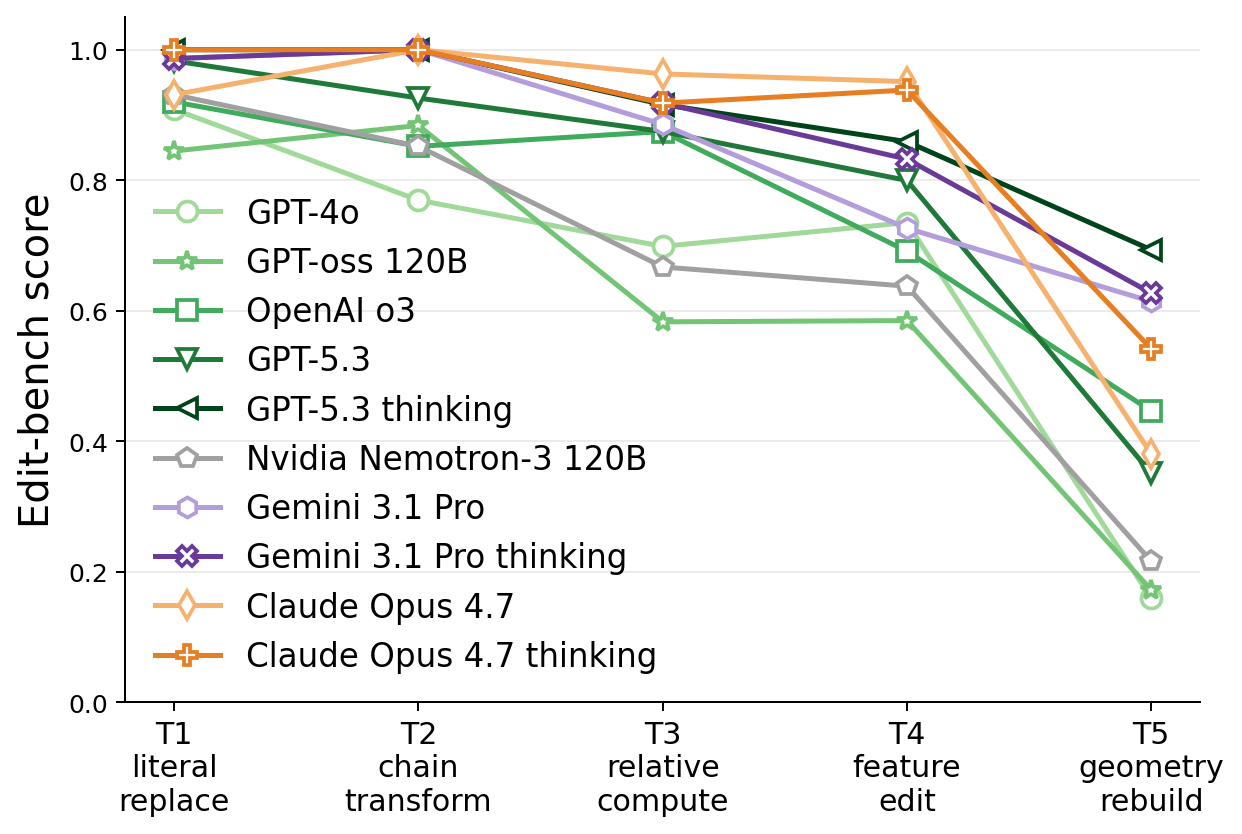
\includegraphics[width=\linewidth]{figures/fig_5.png}   \captionof{figure}{\textbf{BenchCAD-Edit by task type.}}
    \label{fig:edit_task}
  \end{minipage}\hfill                                        \begin{minipage}{0.4\linewidth}                                 \centering                                                    \captionof{table}{\textbf{BenchCAD-Edit Accuracy.}}
    \label{tab:edit_leaderboard}                                \small
\setlength{\tabcolsep}{3pt}
\begin{tabular}{@{}lccc@{}}
\toprule
\textbf{Model}& \textbf{Thinking} & \textbf{Acc.} \\
\midrule
GPT-5.3            & \cmark & \textbf{0.865} \\
Claude Opus 4.7    & \cmark & 0.853 \\
Gemini 3.1 Pro     & \cmark & 0.837 \\
Claude Opus 4.7    & --     & 0.811 \\
Gemini 3.1 Pro     & --     & 0.795 \\
GPT-5.3            & --     & 0.740 \\
OpenAI o3          & \cmark & 0.708 \\
GPT-4o             & --     & 0.615 \\
Nemotron-3 120B    & --     & 0.608 \\
GPT-oss 120B       & --     & 0.561 \\
Baseline (no change) & --     & 0.000 \\
\bottomrule
\end{tabular}
  \end{minipage}
\end{figure} 

\paragraph{\textsc{Code Edit}.} 
\paragraph{Code editing.}
Table~\ref{tab:edit_leaderboard} reports the BenchCAD-Edit leaderboard using mean-normalized improvement as the headline metric, which discounts the varying difficulty of each edit pair. Overall scores show a clear gap between model families, but the per-type breakdown in Fig.~\ref{fig:edit_task} reveals a more diagnostic pattern: simple API-level edits are nearly solved by modern models, while compositional edits remain difficult. The error analysis below ties each regime to specific failure modes; per-model F-code distributions, the full L1--L4 attribution, and the image-conditioned variant are deferred to Appendix~\ref{app:edit_protocol}.


\subsection{Error Analysis}
\label{sec:results_failure_analysis}
\label{sec:exp_failure_analysis}

\begin{wrapfigure}{r}{0.38\linewidth}
  \vspace{-\baselineskip}
  \centering
  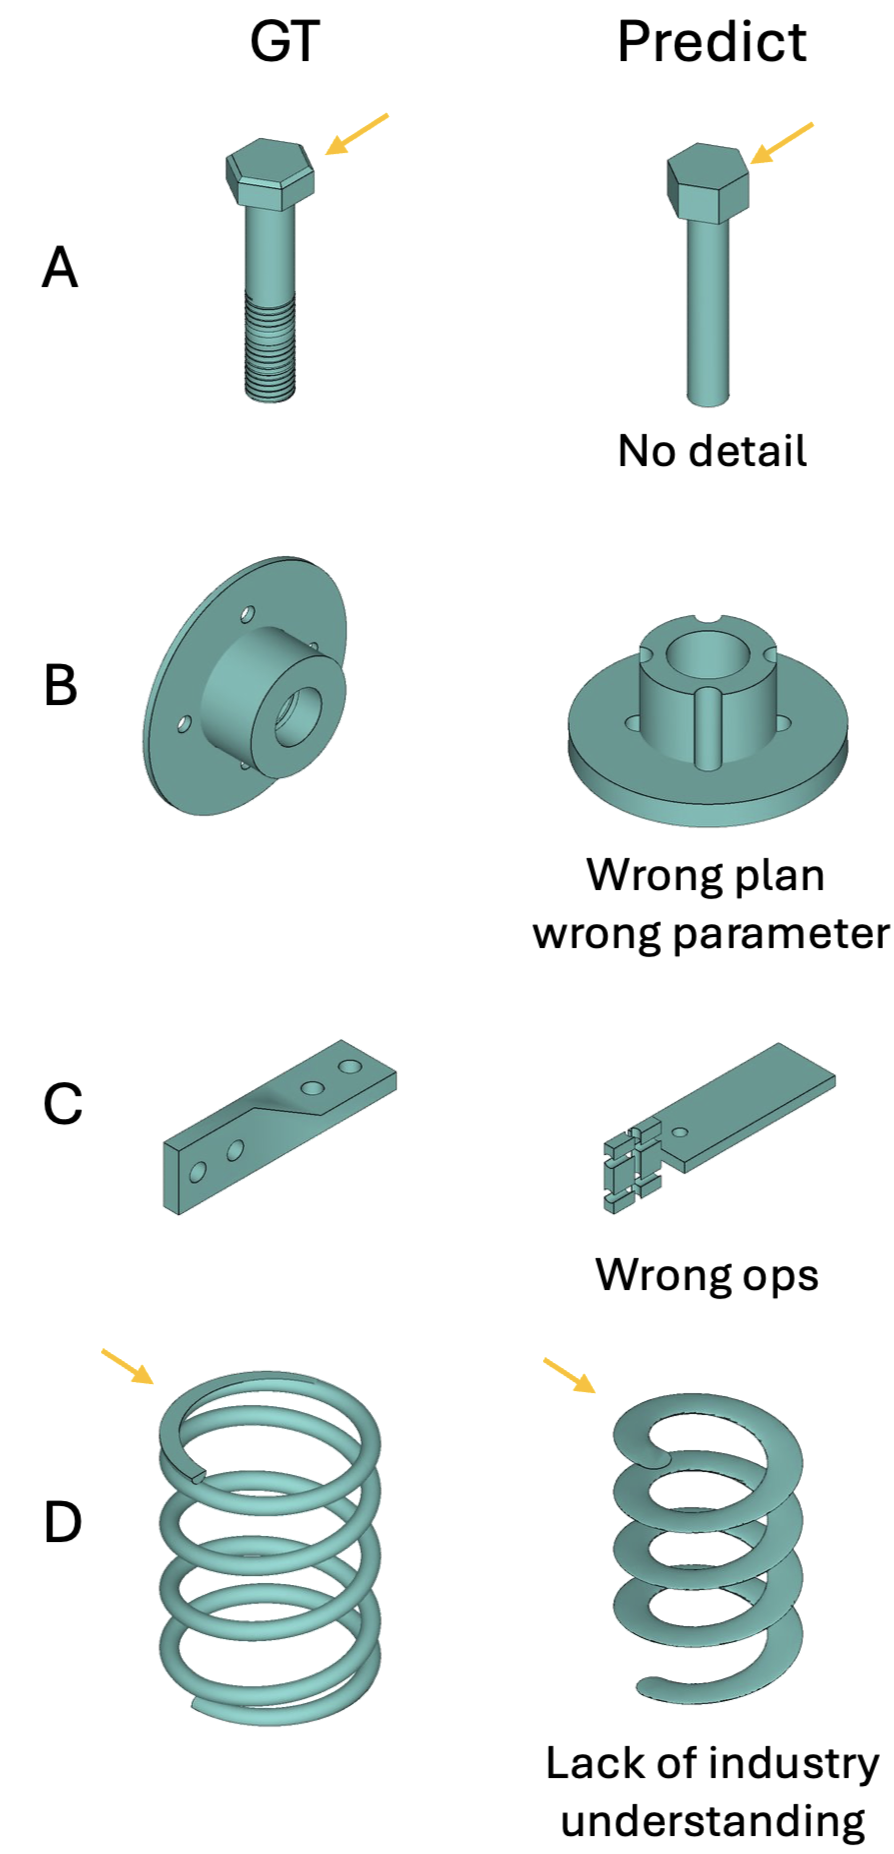
\includegraphics[width=\linewidth]{figures/fig_err_analysis_code_gen.png}
  \caption{\textbf{Examples of failures in codegen.} Zoom-in for more details.}
  \label{fig:err_analysis_codegen}
  \vspace{-0.5\baselineskip}
\end{wrapfigure}

Across tasks, we find that many failures share common causes. Most can be attributed to deficiencies in four core capabilities.


\textbf{Holistic Spatial Recognition}
Visual recognition failures occurs: detailed feature counting and spatial grounding. 
% For instance, 4 out of 8 models fail to identify the keyway adjacent to the central hole in a gear, as the two features are visually blended together in the rendered view.

A hex-head bolt (Figure~\ref{fig:err_analysis_codegen}A) illustrates a fine-detail failure. 
GPT-5.3 recovers the overall bolt body, but omits the threaded shank and chamfered head details. 
The generated part is therefore visually similar at a coarse level but misses small, human-obvious CAD features. 
Consistently, GPT-5.3-chat fails to identify the number of chamfer operations in the corresponding vision QA ($L_1$) on chamfer number. 
Interestingly, though GPT-5.3-thinking answers the chamfer-count question correctly, yet still fails to realize the detail in executable code, suggesting a gap between recognizing a local feature and synthesizing it constructively.

A bearing retainer cap (Figure~\ref{fig:err_analysis_codegen}B) exposes a global spatial-frame failure. 
The model captures several detailed features, but fails to infer the correct extrusion direction: its emitted code extrudes from the XY plane rather than the natural XZ plane. 
This failure is partially diagnosed by the substantially higher 24-axis rotation-invariant IoU compared with the single-axis IoU, indicating that the geometry is partly correct but placed in the wrong spatial frame (\S\ref{app:iou}). 
The same example also reveals parametric-abstraction failures across multiple features.

\textbf{Operation understanding.} A twisted bracket (Figure~\ref{fig:err_analysis_codegen}C) is generated as two mutually perpendicular brackets without twisted connection; the requisite twist-extrusion is absent from the emitted program entirely. 
The model recognizes the holistic spatial (L1) but fails to map the visible torsion to the corresponding CAD operation, exposing an Op Vocabulary Gap (\S\ref{app:op_gap_full}) at the operation-understanding layer.

\textbf{Industrial Parametric abstraction.}
A standardized DIN~2095 coil spring (Figure~\ref{fig:err_analysis_codegen}D) exposes a parametric-abstraction failure. 
The standard requires closed and ground ends: the coil pitch is locally reduced near both terminals, causing the end turns to flatten into planar bearing surfaces. 
The model recognizes the spring and the coil pitch is not a circle, and emits a helical sweep, but collapses this end-specific pitch variation into a uniform helix with an incorrect cross-section.
It therefore captures the coarse family and operation (L1 \& L2) while missing the standard-driven parameterization that an engineer would explicitly encode. 
This failure highlights why BenchCAD anchors its families to engineering standards: the benchmark tests not only whether models can name a part or invoke the right CAD operation, but whether they can recover the structured design rules underlying real parametric CAD.

These cases illustrate how the layered framework converts \textsc{Vision2Code} failures from a single opaque ``wrong code'' category into level-attributable diagnostics: a model can succeed at $L_1$ yet fail at $L_2$ (the bracket), or succeed at $L_1$ and $L_2$ yet fail at $L_3$ (the spring). Without per-level attribution these distinctions collapse into a single low IoU score, and the corresponding training signal --- which level to strengthen --- is lost.

% \textbf{Visual and Code
% Recognition.} Visual recognition failures happen along three axes: detailed feature counting, CAD feature recognition, and spatial grounding. QA asks whether a gear has a keyway, 4/8 models do not find the keyway next to the central cavity.


% We analyze holistic visual recognition failures along three axes: feature counting, CAD feature recognition, and spatial grounding. Models often recognize the presence of repeated structures but fail to count them accurately, especially when they are small, occluded, or densely arranged. They also confuse CAD feature types, such as slots versus holes or protrusions versus cutouts, indicating that coarse silhouette recognition does not imply constructive-geometry understanding. Spatial errors, including misunderstanding the construction plane and rotation axis, as well as incorrect alignment or symmetry judgments, further suggest weak 3D grounding. 



%\textbf{Industrial Parametric Abstraction.} 

%\textbf{Spatial/Code Reasoning.}


%\paragraph{Edit failure-mode breakdown.} A failure-code breakdown (E001--E004 defined in Table~\ref{tab:error_codes}; per-model distribution in Fig.~\ref{fig:edit_error_pies}) shows the dominant failure shifts with model class: \texttt{gpt-4o} and \texttt{gpt-oss-120b} are bottlenecked by \emph{wrong\_operation} (real API, wrong selector or argument); reasoning-tier models trade hallucinations for \emph{no\_op} edits in which the agent rewrites the original byte-for-byte.

%\paragraph{Family Cliff.} Table~\ref{tab:family_cliff} stratifies \texttt{img2cq} pass rate by family difficulty tier. The strongest model collapses by 48\,pt from easy (68\%) to hard (20\%), exhibiting a \textbf{Family Cliff}: hard-tier families exercise advanced operations (helical sweeps, twist-extrusion, lofted Booleans) scarcely present in any prior CAD training corpus, and enforce parametric constraints (gear module--tooth--pitch consistency, spring free-length--turn-count coupling) no model evaluated reliably preserves.

\subsection{Training Findings}
\label{sec:results_training}
\hc{it's a bit unclear why this paragraph is here.}
Our Qwen3-VL-2B trained on BenchCAD achieves SOTA on the in-distribution code-generation benchmark (CodeGen 0.723). When 10 mechanical families are held out, IID-only SFT + RL still transfers non-trivially to the OOD families, indicating that BenchCAD provides useful inductive signal for unseen mechanical structures. Nonetheless, a substantial IID/OOD gap persists, showing that generalization to unseen mechanical families remains an open problem.

\begin{figure*}[t]
  \centering
  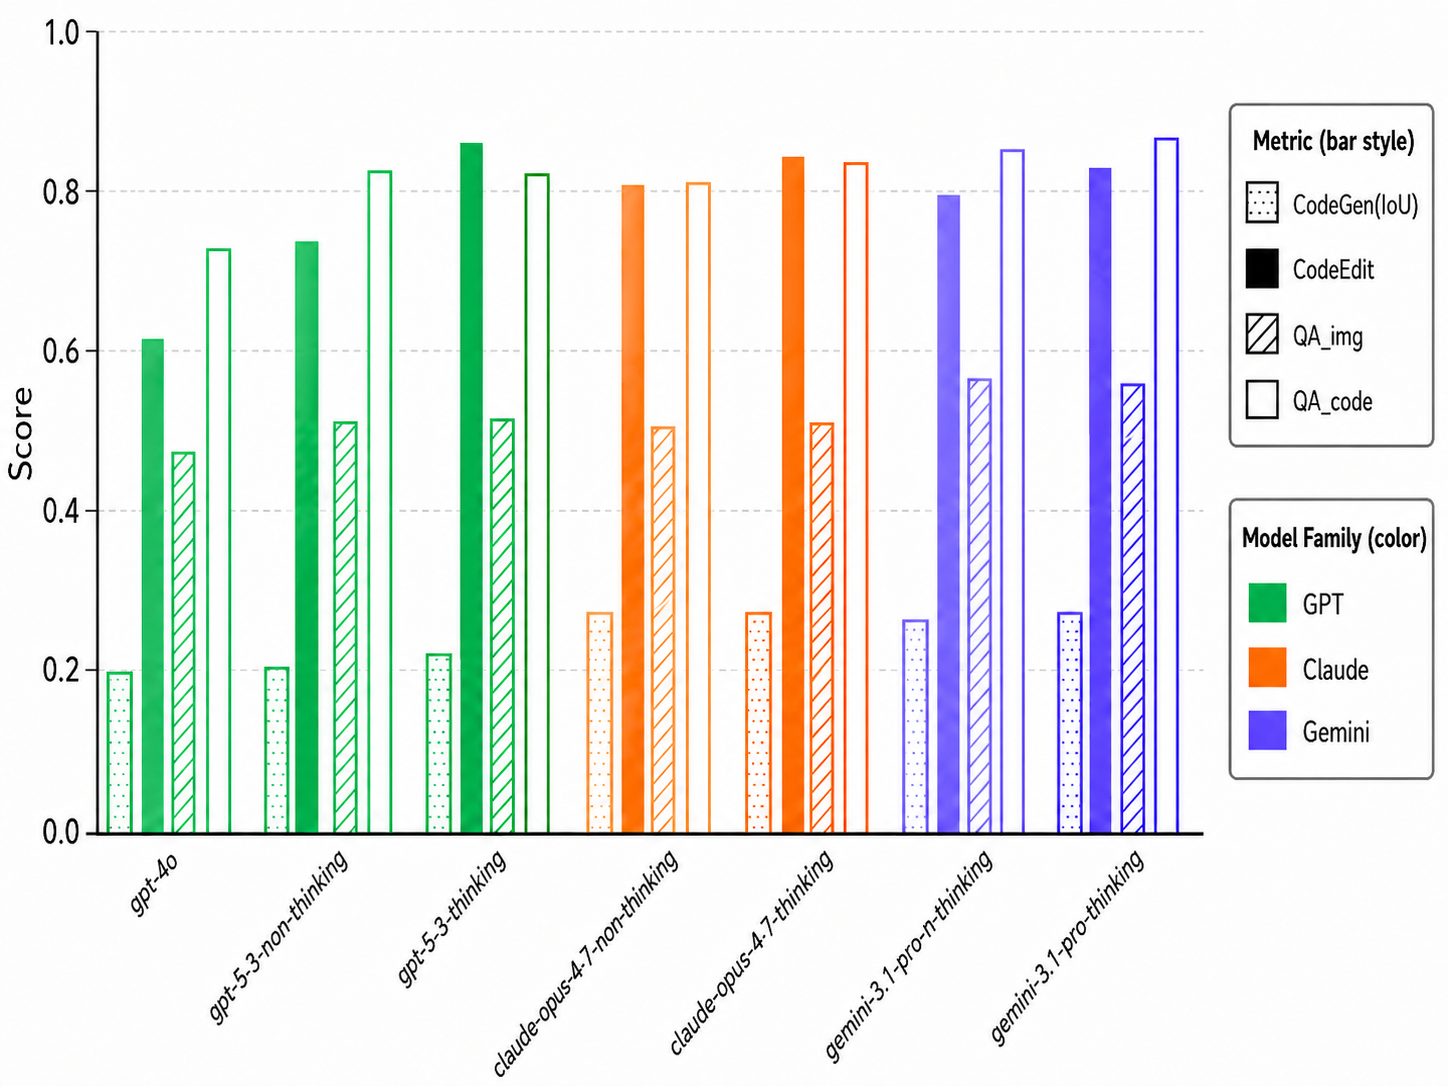
\includegraphics[width=0.65\linewidth]{figures/fig_3.png}
  \caption{\textbf{Per-model performance across the four BenchCAD task categories}
  (frontier proprietary subset; open-source baselines are reported in Table~\ref{tab:main_eval_qa_img}). 
  Bar style encodes task, color encodes model family, and within-family variants distinguish thinking from non-thinking models. 
  Two patterns motivate our subsequent diagnostics: (i) QA-img consistently underperforms QA-code, highlighting the difficulty of holistic spatial recognition from visual evidence; and (ii) CodeEdit trails CodeGen across all models, indicating that instruction-guided modification of existing CAD programs remains harder than greenfield generation.} 
  \label{fig:overall_perform}
\end{figure*}
